% Created 2021-10-06 mar 13:05
% Intended LaTeX compiler: pdflatex
%%% Local Variables:
%%% LaTeX-command: "pdflatex --shell-escape"
%%% End:
\documentclass[11pt]{article}
\usepackage[utf8]{inputenc}
\usepackage[T1]{fontenc}
\usepackage{graphicx}
\usepackage{grffile}
\usepackage{longtable}
\usepackage{wrapfig}
\usepackage{rotating}
\usepackage[normalem]{ulem}
\usepackage{amsmath}
\usepackage{textcomp}
\usepackage{amssymb}
\usepackage{listings}
\usepackage{capt-of}
\usepackage{hyperref}
\hypersetup{colorlinks=true, linkcolor=black}
\setlength{\parindent}{0in}
\usepackage[margin=1.1in]{geometry}
\usepackage[spanish]{babel}
\usepackage{mathtools}
\usepackage{palatino}
\usepackage{fancyhdr}
\usepackage{sectsty}
\usepackage{engord}
\usepackage{cite}
\usepackage{graphicx}
\usepackage{setspace}
\usepackage[compact]{titlesec}
\usepackage[center]{caption}
\usepackage{placeins}
\usepackage{tikz}
\usetikzlibrary{positioning}
\usetikzlibrary{bayesnet}
\usetikzlibrary{shapes.geometric}
\usetikzlibrary{decorations.text}
\usepackage{color}
\usepackage{amsmath}
\usepackage{minted}
\usepackage{pdfpages}

\def\inline{\lstinline[basicstyle=\ttfamily,keywordstyle={}]}

\titlespacing*{\subsection}{0pt}{5.5ex}{3.3ex}
\titlespacing*{\section}{0pt}{5.5ex}{1ex}
\author{José Antonio Álvarez Ocete\\ Francisco Javier Sáez Maldonado}
\date{\today}
\title{Introducción a Hadoop y Spark\\\medskip
\large Procesamiento de Datos a Gran Escala}
\begin{document}

\maketitle

\tableofcontents

\section{Hadoop}

En esta primera sección realizamos diversos experimentos y contestamos a las preguntas planteadas en la práctica.

\subsection{Proceso}

Comenzamos explicando el proceso seguido a partir de la máquina virtual proporcionada para reproducir estos experimentos. En primer lugar, instalamos Java:

\begin{minted}[linenos]{bash}
yum install java-1.8.0-openjdk-devel
\end{minted}

A continuación, cambiamos la versión por defecto que se usaba en las transparencias. Incluso si instalamos la versión 1.7 se instalará la versión 1.8. Hemos de cambiar los paths a las versión 1.8 para que funciona correctamente:

\begin{minted}[linenos]{bash}
export JAVA_HOME=/usr/lib/jvm/jre-1.8.0-openjdk
\end{minted}

Editamos el archivo \inline{/opt/hadoop/etc/hadoop/hadoop.env.sh} añadiendo el \inline{JAVA_HOME}:

\begin{minted}[linenos]{bash}
export JAVA_HOME=/usr/lib/jvm/jre-1.8.0-openjdk
\end{minted}

\subsubsection*{ Compilación}

Tomamos el script proporcionado para compilación y lo ejecutamos utilizando la siguiente orden:

\begin{minted}[linenos]{bash}
./compilar.sh WordCount
\end{minted}

\subsubsection*{ Ejecución }

En primer lugar hemos de iniciar el \emph{NameNode} y el \emph{DataNode}:

\begin{minted}[linenos]{bash}
sbin/start-dfs.sh
\end{minted}

Así como el \emph{ResourceManager} y el \emph{NodeManager}:

\begin{minted}[linenos]{bash}
sbin/start-yarn.sh
\end{minted}

También hemos de subir los archivos de entrada de nuestros programas al sistema de archivo de Hadoop. Para ello utilizamos la siguiente orden:

\begin{minted}[linenos]{bash}
/opt/hadoop/bin/hdfs dfs -put Quijote.txt /user/root
\end{minted}

Finalmente, lanzamos nuestro trabajo de MapReduce:

\begin{minted}[linenos]{bash}
sudo /opt/hadoop/bin/hadoop jar WordCount.jar uam.WordCount Quijote.txt output/
\end{minted}

\subsubsection*{ Resultados }

Obtenemos en el directorio output dos archivos de salida:

\begin{itemize}
	\item Un archivo \inline{SUCCESS} indicando que la tarea ha sido exitosa.
	\item Un archivo \inline{part-r-00000} que tiene la salida del programa que queríamos ejecutar.
\end{itemize}

Mostramos una parte del fichero para ser conscientes de la salida obtenida:

\begin{minted}[linenos]{bash}
"Tablante",	1
"dichosa	1
"el	8
"y	1
(Y	1
(a	1
(al	1
(como	1
(creyendo	1
(de	2
(por	2
(porque	2
(pues	1
(que	21
\end{minted}

Como podemos comprobar, las palabras quedan con ciertos símbolos de puntuación que no deberían ser parte de las palabras. Este repercuteo en un incorrecto conteo. 

\subsubsection*{ Modificación del programa }

Para arreglar esto, basta con cambiar una linea en la función \inline{Map} del archivo \inline{WordCount.java}. En concreto, la modificamos de la siguiente forma:

\begin{minted}[linenos]{java}
StringTokenizer itr = new StringTokenizer(value.toString().
        toLowerCase().replaceAll("[^a-z ]", ""));
\end{minted}

Como podemos comprobar, hemos pasado las palabras a minúsculas usando \inline{toLowerCase} y luego hemos eliminado todo aquello que no sean letras usando \inline{replaceAll}.

Una vez realizada esta modificación, debemos compilar de nuevo el programa como lo hemos hecho anteriormente y, seguidamente, ejecutar de nuevo el programa java para que realice el conteo de palabras. En este caso, indicamos que la salida la realice sobre la carpeta \inline{output2/} para tener las dos salidas por separado y poder compararlas. Obtenemos los dos mismos ficheros que anteriormente.

Hecho esto, utilizamos el archivo \inline{script.py} que hemos creado usando \inline{Python}, que toma todas las palabras que hay en los ficheros de salida y el número de veces que aparece cada una, las ordena y toma las 10 primeras para mostrarlas por pantalla.

El resultado que se obtiene es que las palabras son las mismas y prácticamente en el mismo orden, salvo una pequeña variación entre dos de ellas. Podemos verlo gráficamente en la siguiente figura:

\begin{figure}[H]
	\centering
	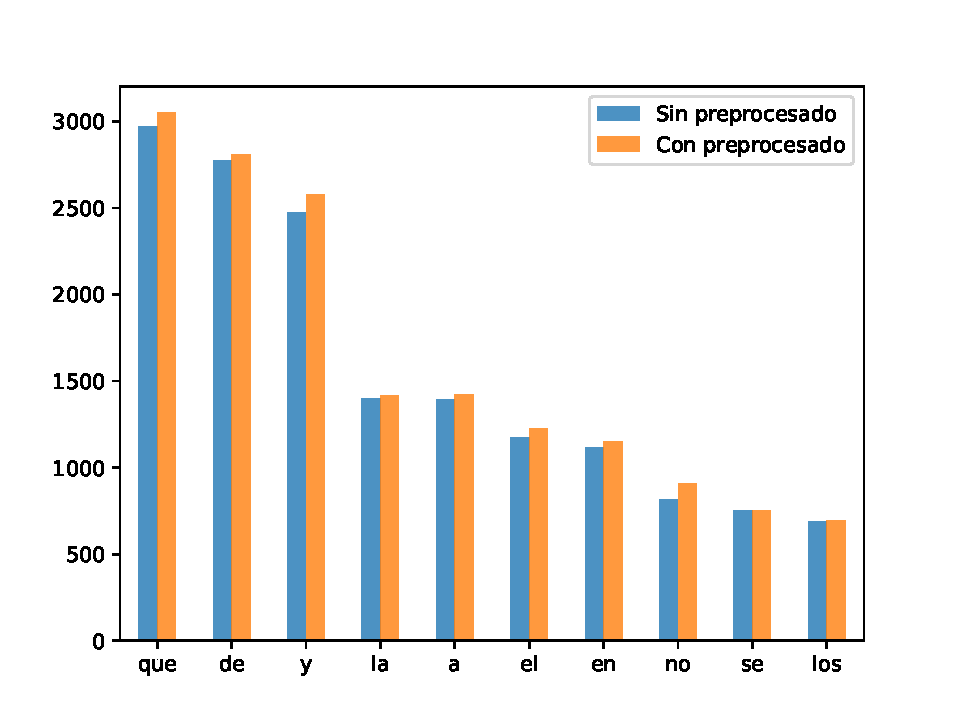
\includegraphics[scale=0.8]{figures/barplot.pdf}
	\caption{Comparación de número de veces que aparece cada palabra con y sin preprocesamiento.}
\end{figure}

Se puede apreciar que, al aplicar el preprocesado, la palabra \inline{a} aparece un número de veces ligeramente superior al que lo hace cuando no tenemos el preprocesador previo del texto.

\subsection{ Cuestiones planteadas}

\subsubsection{ Instalación de Hadoop }

\subsubsection*{ Pregunta 1.1. ¿ Qué ficheros ha modificado para activar la configuración del HDFS? ¿ Qué líneas ha sido necesario modificar? }

Hemos modificado el fichero \inline{/opt/hadoop-2.8.1/etc/hadoop/hadoop-env.sh} añadiendo la línea \inline{export JAVA_HOME= /usr/lib/jvm/jre-1.7.0-openjdk} para especificar la instalación de \inline{Java} que queremos utilizar.

Como se explica en \href{https://stackoverflow.com/questions/17569423/what-is-best-way-to-start-and-stop-hadoop-ecosystem-with-command-line}{esta respuesta de Stack Overflow}, el script \inline{stop-all.sh} detiene todos los daemons de Hadoop a la vez, pero está obsoleto. En lugar de eso es recomendable parar los daemons de HDFS y YARN por separado en todas las máquinas utilizando \inline|stop-dfs.sh| y \inline{stop-yarn.sh}.

A continuación, para instalar Hadoop pseudo-distribuido, hemos modificado el fichero \inline{etc/hadoop/core-site.xml} añadiendo la siguiente propiedad:

\begin{minted}[linenos]{xml}
<configuration>
    <property>
        <name>fs.defaultFS</name>
        <value>hdfs://localhost:9000</value>
    </property>
</configuration>
\end{minted}

Además, añadimos al fichero \inline{/opt/hadoop/etc/hadoop/hdfs-site.xml} lo siguiente:

\begin{minted}[linenos]{xml}
<configuration>
    <property>
        <name>dfs.replication</name>
        <value>1</value>
    </property>
</configuration>
\end{minted}

A continuación, \textbf{para configurar el sistema pseudo-distribuido YARN (y no HDFS)} hemos modificado el fichero \inline{etc/hadoop/mapred-site.xml} añadiendo:

\begin{minted}[linenos]{xml}
<configuration>
    <property>
        <name>mapreduce.framework.name</name>
        <value>yarn</value>
    </property>
</configuration>
\end{minted}

Así como el fichero \inline{etc/hadoop/yarn-site.xml}:

\begin{minted}[linenos]{xml}
<configuration>
    <property>
        <name>yarn.nodemanager.aux-services</name>
        <value>mapreduce_shuffle</value>
    </property>
    
    <property>
        <name>yarn.nodemanager.aux-services.mapreduce_shuffle.class</name>
        <value>org.apache.hadoop.mapred.ShuffleHandler</value>
    </property>
</configuration>
\end{minted}

\subsubsection*{ Ejercicio 1.2: Para pasar a la ejecución de Hadoop sin HDFS, ¿ es suficiente con parar el servicio con \inline{stop-dfs.sh}? ¿ Cómo se consigue ? }

No. La ejecución de dicho script únicamente para el servicio HDFS en ejecución. Sin embargo, debido a la configuración realizada previamente esto no es suficiente. Hemos de modificar el archivo \inline{hdfs-site.xml} eliminando la propiedad \inline{dfs.replication}, así como eliminar \inline{fs.defaultFS} del archivo \inline{core-site.xml}.

\subsubsection{ Ejecución de WordCount }

\subsubsection*{ Pregunta 3.1: ¿ Dónde se crea hdfs ? ¿ Cómo se puede decidir su localización ? }

El sistema de archivos HDFS se crea donde la variable \inline{dfs.datanode.data.dir} indique. Esta variable se puede modificar en el archivo \inline{hdfs-site.xml}. \href{https://hadoop.apache.org/docs/r2.4.1/hadoop-project-dist/hadoop-hdfs/hdfs-default.xml}{Su valor por defecto} es
\begin{minted}[linenos]{bash}
file://${hadoop.tmp.dir}/dfs/data
\end{minted}
y, podemos ver que la variable \inline{hadoop.tmp.dir} tiene el valor \inline{/tmp/hadoop-\${user.name}} .

\subsubsection*{ Pregunta 3.2: ¿ Cómo se puede borrar todo el contenido del HDFS, incluido su estructura ?}

Si con \emph{todo el contenido} nos referimos a una desistalación completa podemos seguir \href{https://medium.com/@deepeshtripathi/completely-uninstall-and-delete-hadoop-from-hosts-hortonworks-1a3f755afa20}{este post en Medium} para realizar un borrado completo de Hadoop, incluyendo servicios, logs, paquetes, dependencias innecesarias, y cualquier otro tipo de referencia en nuestro sistema a Hadoop.

Por otro lado, para borrar toda la estructura interna de archivos de HDFS podemos utilizar el comando:

\begin{minted}[linenos]{bash}
bin/hdfs dfs -rm -R /
\end{minted}

\subsubsection*{ Pregunta 3.3: Si estás usando hdfs, ¿ cómo puedes volver a ejecutar WordCount como si fuese single.node ? }

Recordamos que hemos hecho una serie de cambios en archivos \inline{xml} para configurar Hadood para que funcionase de forma pseudo-distribuida. Para ejecutarlo como si fuese \emph{single-node}, deberíamos eliminar los cambios que hemos hecho en estos ficheros \inline{xml}: \inline{core-site.xml} y \inline{hdfs-site.xml}. Así, volveríamos al modo por defecto de Hadoop y conseguiríamos que funcionase como si fuese \inline{single-node}.

\subsubsection*{ Pregunta 3.4: ¿ Cuáles son las 10 palabras más utilizadas ? }

Esta pregunta ya ha sido mostrada anteriormente en la Figura 1. Las palabras más utilizadas son \inline{[que, de , y, la, a, el, en, no, se, los]}

\subsubsection*{ Pregunta 3.5: Cuántas veces aparecen las siguientes palabras: el, dijo }

Para esta pregunta, volvemos a usar nuestro fichero \inline{script.py} que nos imprimirá cuántas veces aparece cada una de ellas en el texto, primero usando preprocesado y a continuación sin utilizarlo.

\begin{minted}[linenos]{bash}
Numero de veces que aparece la palabra
    el
        - Sin preprocesado 1173
        - Con preprocesado 1228
    dijo
        - Sin preprocesado 196
        - Con preprocesado 271
\end{minted}

Puede comprobarse ejecutando el script indicado.

\subsubsection{ Modificación de parámetros MapReduce }

Creamos un archivo con 15 copias del Quijote llamado \inline{quijote15.txt}. Lo subimos al sistema de archivos de hdfs:

\begin{minted}[linenos]{bash}
bin/hdfs dfs -put quijote15.txt /user/root/quijote15-128mb.txt
\end{minted}

A continuación, volvemos a subir el archivo indicando el tamaño de bloque a utilizar, 2MB:

\begin{minted}[linenos]{bash}
	bin/hdfs dfs -D dfs.blocksize=2097152 -put quijote15.txt /user/root/quijote15-2mb.txt
\end{minted}

Por otro lado, también podemos cambiar el valor por defecto del tamaño de bloque para no tener que especificar el tamaño 2MB cada vez que subamos un archivo. Para ello cambiamos el respectivo parámetro (\inline{dfs.block.size}) en los archivos de configuración de hdfs editando \inline{hdfs-site.xml}, añadiendo:

\begin{minted}[linenos]{xml}
<property>
     <name>dfs.block.size</name>
     <value>2097152</value>
</property>
\end{minted}

Y reiniciamos dfs y yarn para asegurarnos que la configuración activa incluye los cambios realizados. Subimos de nuevo el archivo \inline{quijote15.txt} sin especificar el tamaño de bloque utilizando la siguiente orden:

\begin{minted}[linenos]{bash}
bin/hdfs dfs -put quijote15.txt /user/bigdata/dreji/quijote15-2mb-default.txt
\end{minted}

A continuación accedemos a \inline{http://localhost:50070/explorer.html#/user/root} para comprobar los resultados.

\begin{figure}[H]
  \centering
  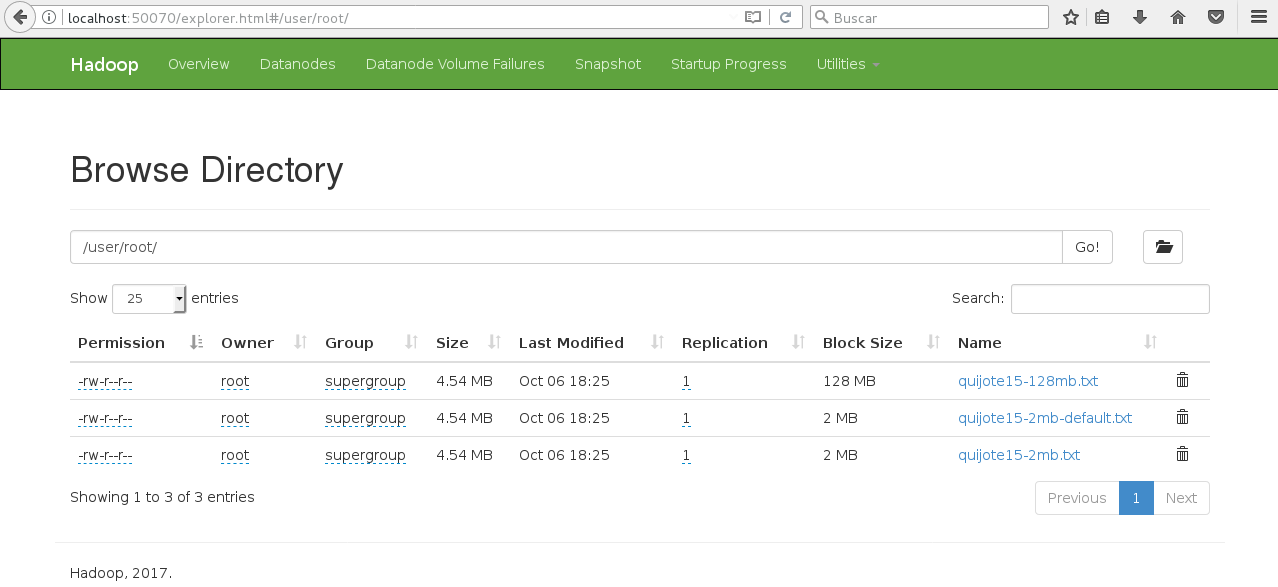
\includegraphics[scale=0.5]{figures/quijote15}
  \caption{Captura del explorador del HDFS de hadoop}
\end{figure}

Podemos comprobar como la primera versión del archivo \inline{quijote15.txt} subida tienen tamaño de bloque de 128MB, mientras que las dos últimas tienen tamño de bloque 2MB. Esto responde a las preguntas 4.1, 4.2 y 4.3 del guión, que nos piden comparar distintas formas de modificar el tamaño de bloque al subir archivos a HDFS.

Procedemos a comparar la ejecución de nuestro programa para distintos tamaños de bloque. Para ello ejecutamos el programa contador de palabras utilizando los archivos de entrada \inline{quijote15-128mb.txt} y \inline{quijote15-2mb.txt} subidos anteriormente. Utilizando 2MB como tamaño de bloque obtenemos la siguiente salida:

\begin{minted}[linenos]{bash}
[...]
Shuffled Maps=3
Merged Map outputs=3
[...]
\end{minted}

Indicando que se han realizado 3 operaciones \emph{map} y 3 operaciones \emph{reduce}. Este número de operaciones encaja con lo esperado, pues el archivo \inline{quijote15.txt} pesa 4.54MB y se divide en tres bloques de 2MB. Al repetir la ejecución con 128MB para el tamaño de bloque obtenemos:

\begin{minted}[linenos]{bash}
[...]
Shuffled Maps=1
Merged Map outputs=1
[...]
\end{minted}

Obteniendo una única operación map y reduce, pues un único bloque de 128MB es suficiente para para el archivo de 4.54MB. De esta forma hemos comprobado como afecta el tamaño de bloque en la ejecución de un programa MapReduce: Afecta al número de bloques creados y, por lo tanto, al nñumero de operaciones map/reduce realizadas.

Las salidas de estas últimas ejecuciones pueden encontrarse en los archivos \inline{output-quijote15-2mb.txt} y \inline{output-quijote15-128mb.txt} respectivamente.


\newpage
\section{ Tutorial de Spark}


En esta segunda parte de la práctica seguiremos el tutorial de spark contestando a las cuestiones planteadas.


\subsubsection*{ Pregunta TS1.1 ¿Cómo hacer para obtener una lista de los elementos al cuadrado?}

Bastará en este caso usar sobre el RDD la función map pasándole como parámetro la función \inline{lambda x: x*x} que eleva el número al cuadrado. 
A continuación vemos el código con su respectiva salida:

\begin{minted}[linenos]{python}
numeros = sc.parallelize([1,2,3,4,5,6,7,8,9,10])
cuadrados = numeros.map(lambda x : x*x)
print(cuadrados.collect())

[1, 4, 9, 16, 25, 36, 49, 64, 81, 100]
\end{minted}

\subsubsection*{ Pregunta TS1.2 ¿Cómo filtrar los impares? }

Utilizando sobre el RDD la función \inline{filter} proporcionándole como parámetro la función que calcula si cada elemento es impar, esto es, si su módulo 2 es 1 : \inline{lambda x : x\%2 == 1}. El código completo es el siguiente:

\begin{minted}[linenos]{python}
rddi = numeros.filter (lambda x: x%2==1)
print (rddi.collect())

[1, 3, 5, 7, 9]
\end{minted}

\subsubsection*{ Pregunta TS1.3 ¿Tiene sentido esta operación? ¿Si se repite se obtiene siempre el mismo resultado?}

Se nos ha proprocionado el siguiente código:

\begin{minted}[linenos]{python}
#Tiene sentido esta operacion?
numeros = sc.parallelize([1,2,3,4,5])

print (numeros.reduce(lambda elem1, elem2: elem1-elem2))
\end{minted}

Esta operacion no tiene sentido, pues para hacer el reduce necesitamos que la operación sea conmutativa, es decir, que $a-b = b-a$. Esto \textbf{no} es cierto para la operación diferencia en todos los casos. Es por ello que no se producirán siempre los mismos resultados. Basta con ejecutar el código múltiples ocasiones para ver cómo varían los resultados.

\subsubsection*{ Pregunta TS1.4 ¿Cómo lo ordenarías para que primero aparezcan los impares y luego los pares?}

Lo haremos para el caso general. Utilizaremos el método \inline{takeOrdered()}, al que le pasamos el número de elementos a tomar y una función de ordenación. Para calcular el número de elementos basta con utilizar el método \inline{count()}.

Por otro lado, como función de ordenación utilizaremos \inline{lambda x: x\%2 == 0}, que asigna un mayor valor a los nñumeros impares (1) y uno menor a los pares (0). Puesto que \inline{takeOrdered} ordena descendentemente, los números impares aparecerán antes que los pares. El código final es el siguiente:

\begin{minted}[linenos]{python}
numeros = sc.parallelize([3,2,1,4,5])
n = numeros.count()
print(numeros.takeOrdered(n,lambda elem: elem%2== 0))

[3, 1, 5, 2, 4]
\end{minted}

\subsubsection*{ Pregunta TS1.5 ¿Cuántos elementos tiene cada rdd? ¿Cuál tiene más? }

Se nos proporciona el sigueinte código:

\begin{minted}[linenos]{python}
lineas = sc.parallelize(['', 'a', 'a b', 'a b c'])

palabras_flat = lineas.flatMap(lambda elemento: elemento.split())
palabras_map = lineas.map(lambda elemento: elemento.split())

print (palabras_flat.collect())
print (palabras_map.collect())
\end{minted}

Cuya salida es:

\begin{minted}[linenos]{python}
['a', 'a', 'b', 'a', 'b', 'c']
[[], ['a'], ['a', 'b'], ['a', 'b', 'c']]
\end{minted}

Para contar los elementos de cada RDD podemos volver a utilizar \inline{count()}:

\begin{minted}[linenos]{python}
print(palabras_flat.count())
print(palabras_map.count())

6
4
\end{minted}

Como podemos ver, \inline{palabras_flat} tiene más elementos. Esto ocurre porque en \inline{flatMap} cada elemento de entrada al que se le aplica la función \inline{lambda} puede tener como salida 0 o más (un vector) de elementos. Por tanto:

\begin{itemize}
	\item Con \inline{flatMap}, para cada elemento de \inline{lineas} obtenemos un vector que luego separaremos por elementos e ignoraremos los elementos que estén vacíos. Por ello, de 4 elementos iniciales pasamos a 6 que es el total de letras que tenemos en el RDD.
	
	\item Con \inline{map}, a cada uno de los vectores iniciales se le aplica la función indicada y se introducen el resultado en un vector. El resultado final esun vector con cada uno de esos vectores. Es por ello que al ejecutar \inline{map} siempre obtendremos un RDD con tantos vectores como elementos había en el RDD de entrada.
\end{itemize}

\subsubsection*{ Pregunta TS1.6 ¿De qué tipo son los elementos del rdd \inline{palabras\_map}? ¿Por qué \inline{palabras\_map} tiene el primer elemento vacío?}

Siguiendo la respuesta de la pregunta anterior, en \inline{palabras_map} obtenemos un vector tras aplicar la función a cada elemento de \inline{lineas}, por lo que los elementos de \inline{palabras_map} son vectores. Lo podemos ver en la salida del siguiente código:

\begin{minted}[linenos]{python}
print (palabras_map.collect())

[[], ['a'], ['a', 'b'], ['a', 'b', 'c']]
\end{minted}

Además, tiene el primer \textbf{elemento vacío} porque la función split aplicada sobre el elemento \inline{''} devuelve un vector vacío pues no hay nada que separar.

\subsubsection*{ Pregunta TS1.7. Prueba la transformación \inline{distinct} si lo aplicamos a cadenas.}

Para probarlo, ejecutamos el siguiente código en el que ponemos en un RDD ejemplos de prueba con las mismas palabras en mayúscula y minúscula, con espacios o signos de puntuación:

\begin{minted}[linenos]{python}
test = sc.parallelize(["abcd", "abcd","dcba","abCd","a bcd","hola",
        "HOLA","hola!","HoLa","ho la"])

dis = test.distinct()

print(dis.collect())
\end{minted}

La salida que obtenemos es:

\begin{minted}[linenos]{python}
['abcd', 'abCd', 'a bcd', 'hola', 'hola!', 'dcba', 'HOLA', 'HoLa', 'ho la']
\end{minted}

Como podemos ver, teníamos un único ejemplo duplicado (el primero) que es el único que se ha eliminado. Esto nos indica que el comparador de elementos de los rdd comparan los strings \textbf{caracter a caracter}.

\subsubsection*{ Pregunta TS1.8 ¿Cómo se podría obtener la misma salida pero utilizando una sola transformación y sin realizar la unión?}

Se podría hacer que el filtro se quede con los elementos que empiecen por I o por E, haciendo el código del siguiente modo:

\begin{minted}[linenos]{python}
log = sc.parallelize(['E: e21', 'I: i11', 'W: w12', 'I: i11',
                     'W: w13', 'E: e45'])

inferr = log.filter(lambda elem: elem[0] in ['I','E'])
print(inferr.collect())

'E: e21', 'I: i11', 'I: i11', 'E: e45']
\end{minted}

\subsubsection*{ Pregunta TS1.9 ¿Cómo explica el funcionamiento de las celdas anteriores?}

Comentamos una a una las celdas anteriores:

\begin{minted}[linenos]{python}
numeros = sc.parallelize([1,2,3,4,5])

print (numeros.reduce(lambda elem1,elem2: elem2+elem1))
\end{minted}

Esta primera celda solo crea un RDD y luego hace la operación reduce, que combina los valores usando una función que le indicamos, en este caso la suma de los valores. Así, devolverá la suma de todos los valores ya que esta operación es conmutativa y asociativa.

\begin{minted}[linenos]{python}
#Tiene sentido esta operacion?
numeros = sc.parallelize([1,2,3,4,5])

print (numeros.reduce(lambda elem1,elem2: elem1-elem2))
\end{minted}

Esta celda hace lo mismo que la anterior salvo que la operación que realiza es la resta. Como ya hemos visto en una pregunta anterior, esta operación no tiene sentido pues la resta no es una operación conmutativa por lo que el resultado no siempre será el mismo.

\begin{minted}[linenos]{python}
palabras = sc.parallelize(['HOLA', 'Que', 'TAL', 'Bien'])

pal_minus = palabras.map(lambda elemento: elemento.lower())

print (pal_minus.reduce(lambda elem1,elem2: elem1+"-"+elem2))
#y esta tiene sentido esta operacion?
# Que pasa si ponemos elem2+"-"+elem1
\end{minted}

En esta celda se crea un RDD que tiene cadenas de caracteres, primero se pasan a minúsculas aplicándoles la funcion \inline{.lower} y luego se concatenan todas las palabras a un solo scring uniéndolas por guiones, obteniendo como salida:

\begin{minted}[linenos]{bash}
hola-que-tal-bien
\end{minted}

Si cambiásemos el orden en el que se concatenan los elementos como se nos indica en el comentario, la salida cambia y las palabras se van uniendo en el orden inverso, debido a cómo se realiza la operación reduce. La salida es:

\begin{minted}[linenos]{bash}
bien-tal-que-hola
\end{minted}

\begin{minted}[linenos]{python}
r = sc.parallelize([('A', 1),('C', 4),('A', 1),('B', 1),('B', 4)])
rr = r.reduceByKey(lambda v1,v2:v1+v2)
print (rr.collect())
\end{minted}

En esta celda se crea un RDD que tiene como elementos Tuplas \inline{(clave,valor)}. A continuación, usando \inline{reduceByKey} pasándole como argumento una función suma, lo que se hace es sumar los valores de las tuplas cuya clave sea la misma, obteniendo la salida esperada:

\begin{minted}[linenos]{bash}
[('C', 4), ('A', 2), ('B', 5)]
\end{minted}

La última celda es la siguiente:

\begin{minted}[linenos]{python}
r = sc.parallelize([('A', 1),('C', 4),('A', 1),('B', 1),('B', 4)])
rr1 = r.reduceByKey(lambda v1,v2:v1+v2)
print (rr1.collect())
rr2 = rr1.reduceByKey(lambda v1,v2:v1)
print (rr2.collect())
\end{minted}

De nuevo, se crea un RDD cuyos elementos son tuplas \inline{(clave,valor)} , primero se realiza lo mismo que en la celda anterior, y luego se vuelve a aplicar sobre el RDD obtenido la función \inline{reduceByKey} esta vez pasándole como función simplemente mantenerla clave que tiene. Sin embargo, esto no parece producir ningún efecto sobre el RDD, pues cuando se realiza la operación \inline{collect} para ver los elementos del mismo, la salida es la misma que se produce en la celda anterior.

Como \textbf{conclusión} a esta pregunta, podemos decir que es importante cómo se aplica la función \inline{reduce} sobre los RDD y que hay que tener cuidado con las operaciones que indicamos a esta función pues podrían no producir los resultados que se desean. 

\subsubsection*{ Pregunta \inline{groupByKey}}

Dada la siguiente celda

\begin{minted}[linenos]{python}
r = sc.parallelize([('A', 1),('C', 2),('A', 3),('B', 4),('B', 5)])
rr = r.groupByKey()
res= rr.collect()

print(rr.collect())

# Que operacion realizar al RDD rr para que la operacion sea como un reduceByKey
\end{minted}

Lo primero que vemos es que la operación \inline{rr.collect} devuelve una lista con tuplas \inline{(clave, pyspark Result Iterable)}. Estos iterables debemos pasarlos primero a una lista, y luego realizar sobre ellos la operación que quisiésemos hacer con el \inline{reduceByKey}. Vemos que los pasamos a una lista utilizando \inline{mapValues(list)} que convierte los valores a un tipo:

\begin{minted}[linenos]{python}
rrf = rr.mapValues(list).collect()
print(rrf)

[('C', [2]), ('A', [1, 3]), ('B', [4, 5])]
\end{minted}

Y, a continuación, podemos realizar la operación que haríamos con el reduce. Por ejemplo, si queremos hacer la suma de los vectores utilizando \inline{map} podríamos hacer todo en una linea de la siguiente manera:

\begin{minted}[linenos]{python}
rrf = rr.mapValues(list).map(lambda x : (x[0],sum(x[1])))
print(rrf.collect())

[('C', 2), ('A', 4), ('B', 9)]
\end{minted}

Ahora, se nos pide simular el \inline{groupByKey} usando \inline{reduceByKey} y \inline{map}. Para ello, usando \inline{reduceByKey} podemos obtener las listas que obtendríamos tras aplicar el \inline{mapValues(list)} que hemos obtenido anteriormente.

\begin{minted}[linenos]{python}
simul_group = r.reduceByKey(lambda v1,v2: [v1,v2])
print(simul_group.collect())

[('C', 2), ('A', [1, 3]), ('B', [4, 5])]
\end{minted}

\subsubsection*{ Pregunta sobre \inline{join}}

\begin{minted}[linenos]{python}
rdd1 = sc.parallelize([('A',1),('B',2),('C',3)])
rdd2 = sc.parallelize([('A',4),('B',5),('C',6)])

rddjoin = rdd1.join(rdd2)
\end{minted}

El resultado de esto es:

\begin{minted}[linenos]{bash}
[('A', (1, 4)), ('B', (2, 5)), ('C', (3, 6))]
\end{minted}

Es decir, un nuevo RDD en el que los valores son tuplas con los valores que hay en cada uno de los RDD. Se nos pide que, dado ese código, cambiemos las claves de los dos RDDs iniciales para ver qué RDD se crea finalmente. Si lo hacemos, cambiando por ejemplo los RDD del siguiente modo:

\begin{minted}[linenos]{python}
rdd1 = sc.parallelize([('A',1),('B',2),('D',3)])
rdd2 = sc.parallelize([('A',4),('B',5),('E',6)])

rddjoin = rdd1.join(rdd2)
\end{minted}

El resultado obtenido es el siguiente:

\begin{minted}[linenos]{bash}
[('A', (1, 4)), ('B', (2, 5))]
\end{minted}

Es decir, que el \inline{join} está haciendo la unión de los elementos cuyas claves están en la intersección del conjunto de claves. Como \inline{D} y \inline{E} no están en ambos RDD, no están en la intersección del conjunto de claves y por tanto no se obtienen en el RDD final.

\subsubsection*{ Tipos de Join }

Se nos pregunta que qué ocurre cuando sustituimos \inline{join} por \inline{leftOuter/rightOuter/fullOuter} join. El resultado es que estos tipos de \inline{join} crean elementos en el nuevo RDD aunque sus claves no estén en ambos RDD iniciales. En concreto:

\begin{itemize}
		\item \inline{leftOuter} añade al nuevo RDD también las tuplas \inline{(clave,valor)} cuya clave esté en el \inline{RDD} sobre el que se llama la función, pero no estén en el RDD que se pasa como parámetro. Se añade un \inline{None} en la tupla conjunta del RDD final:
		
		\begin{minted}[linenos]{python}
rdd1 = sc.parallelize([('A',1),('B',2),('C',3)])
rdd2 = sc.parallelize([('A',4),('A',5),('B',6),('D',7)])
rddjoin = rdd1.leftOuterJoin(rdd2)

[('A', (1, 4)), ('A', (1, 5)), ('B', (2, 6)), ('C', (3, None))]
		\end{minted}
	
		\item \inline{rightOuter} hace lo mismo que el anterior pero en el sentido opuesto, es decir, usando el segundo RDD.
		\item \inline{fullOuter} combina los dos anteriores.
\end{itemize}

\subsubsection*{ Pregunta TS1.10 Borra la salida y cambia las particiones en parallelize. ¿ Qué sucede ?}

Lo que ocurre si ponemos 10 particiones es lo siguiente (borrando anteriormente el contenido del directorio donde tenemos la salida):

\begin{minted}[linenos]{python}
numeros = sc.parallelize(range(0,1000),10)
numeros.saveAsTextFile('salida')

%ls -la salida/*

-rw-r--r-- 1 root root 290 Oct  4 10:42 salida/part-00000
-rw-r--r-- 1 root root 400 Oct  4 10:42 salida/part-00001
-rw-r--r-- 1 root root 400 Oct  4 10:42 salida/part-00002
-rw-r--r-- 1 root root 400 Oct  4 10:42 salida/part-00003
-rw-r--r-- 1 root root 400 Oct  4 10:42 salida/part-00004
-rw-r--r-- 1 root root 400 Oct  4 10:42 salida/part-00005
-rw-r--r-- 1 root root 400 Oct  4 10:42 salida/part-00006
-rw-r--r-- 1 root root 400 Oct  4 10:42 salida/part-00007
-rw-r--r-- 1 root root 400 Oct  4 10:42 salida/part-00008
-rw-r--r-- 1 root root 400 Oct  4 10:42 salida/part-00009
-rw-r--r-- 1 root root   0 Oct  4 10:42 salida/_SUCCESS
\end{minted}

Como se podía esperar, se crea un archivo para cada una de las particiones de salida, según el número de particiones que le hayamos indicado.

\subsection{Procesamiento El Quijote}

\subsubsection*{ Pregunta TS2.1 Explica la utilidad de cada transformación y detalle para cada una de ellas si cambia el número de elementos en el RDD resultante. Es decir si el RDD de partida tiene N elementos, y el de salida M elementos, indica si N>M, N=M o N<M.}

Dado el siguiente código:

\begin{minted}[linenos]{python}
charsPerLine = quijote.map(lambda s: len(s))
allWords = quijote.flatMap(lambda s: s.split())
allWordsNoArticles = allWords.filter(lambda a: a.lower() not in ["el", "la"])
allWordsUnique = allWords.map(lambda s: s.lower()).distinct()
sampleWords = allWords.sample(withReplacement=True, fraction=0.2, seed=666)
weirdSampling = sampleWords.union(allWordsNoArticles.sample(False, fraction=0.3))
\end{minted}

Se nos pide indicar qué hace cada una de las transformaciones. Procedemos línea a línea:

\begin{enumerate}
	\item \inline{charsPerLine = quijote.map(lambda s: len(s))} esta línea obtiene un nuevo RDD en el que se cambian las líneas del quijote por la longitud de cada línea. No se modifica el número de elementos, se tiene $N = M$.
	
	\item \inline{allWords = quijote.flatMap(lambda s: s.split())} obtiene un nuevo RDD en el que se separa cada uno de los strings iniciales en cada una de sus palabras y luego cada palabra se convierte en un elemento del RDD. Por tanto, el RDD de salida tiene muchos más elementos que el de entrada, podemos decir que $M >> N$.
	
	\item \inline{allWordsNoArticles = allWords.filter(lambda a: a.lower() not in ["el", "la"])} se toma el RDD de las palabras y se pasa un filtro que elimina todos los artículos *el* y *la* (sin distinción de mayúsculas/minúsculas) del documento. Al eliminar elementos, el número de elementos en la salida será menor que en la entrada por lo que $M < N$.
	
	\item \inline{allWordsUnique = allWords.map(lambda s: s.lower()).distinct()} se crea un RDD que tiene un elemento por cada palabra distinta (sin distinción mayúsculas/minúsculas) que haya en el RDD \inline{allWords}. De nuevo, se eliminan elementos repetidos por lo que el número de elementos en la salida será menor que en la entrada, $M < N$.
	
	\item \inline{sampleWords = allWords.sample(withReplacement=True, fraction=0.2, seed=666)} se extrae aleatoriamente con reemplazamiento un $20\%$ de las palabras que hay en \inline{allWords} para crear un nuevo RDD. Por supuesto, se tendrá que $M = 0.2 N$ ($M < N$).
	
	\item \begin{minted}[linenos]{python}
weirdSampling = sampleWords.union
     (allWordsNoArticles.sample(False, fraction=0.3))
		\end{minted} 
		primero extrae sin reemplazamiento un $30\%$ de elementos que tenemos en el RDD que no tiene artículos (en este caso, tendríamos $M < N$ pues reducimos elementos) y a continuación une estos elementos extraídos al RDD que tiene una muestra del $20\%$ que hemos obtenido en el paso anterior. En esta unión aumenta el tamaño del RDD por lo que en este paso $M > N$.
\end{enumerate}

Ahora, explicamos las funciones en general, su utilidad y si cambia el número de elementos del RDD resultante:

\begin{itemize}
	\item \inline{map} sirve para realizar una transformación sobre el RDD pasándole como parámetro una función. El número de elementos final del RDD es el mismo, pues a cada elemento se le aplica una función pero sigue siendo un elemento, no se elimina ninguno, por lo que $M=N$.
	
	\item \inline{flatmap} realiza una transformación y, a continuación, si tenemos vectores como puntos, hace que cada elemento de los vectores sea un punto del nuevo RDD, por lo que en este caso el número se mantiene (si cada vector de salida tiene dimensión 1), o aumenta, por lo que $M \geq N$.
	
	\item \inline{filter} selecciona un conjunto de elementos según una función que da una condición implícita. Todos los elementos pueden cumplir esa condición o solo un subconjunto de ellos, por lo que $M \leq N$.
	
	\item \inline{distinct} toma los elementos del RDD que sean únicos (diferentes a todos los demás). Todos podrían ser diferentes o podría haber elementos iguales, por lo que $M \leq N$.
	
	\item \inline{sample} toma una muestra del tamaño indicado. En este caso, el RDD no se modifica solo que se toman ejemplos del mismo, por lo que podemos decir que el tamaño del RDD se mantiene, $M=N$.
	
	\item \inline{union} une dos RDDs en uno.
\end{itemize}

\subsubsection*{ Pregunta TS2.2 Explica el funcionamiento de cada acción anterior }

Tenemos el siguiente código:

\begin{minted}[linenos]{python}
numLines = quijote.count()
numChars = charsPerLine.reduce(lambda a,b: a+b) # also charsPerLine.sum()
sortedWordsByLength = allWordsNoArticles.takeOrdered(20, key=lambda x: -len(x))
numLines, numChars, sortedWordsByLength
\end{minted}

Este código hace lo siguiente:

\begin{enumerate}
	\item \inline{numLines = quijote.count()} cuenta el número de líneas que tiene el quijote.
	
	\item \inline{numChars = charsPerLine.reduce(lambda a,b: a+b)} utiliza un RDD anterior que
	tiene el número de caracteres que tiene cada línea y los suma, obteniendo así el número de caracteres total.
	
	\item La siguiente línea
	\begin{minted}[linenos]{python}
sortedWordsByLength = allWordsNoArticles.takeOrdered(20, key=lambda x: -len(x))
	\end{minted} 
	toma el RDD que tiene todas las palabras y toma las 20 palabras que tienen MAYOR longitud
\end{enumerate}

A continuación, se pide que se implemente la acción \inline{count} que nos dice el número de elementos que tiene un RDD usando lo siguiente:
\begin{itemize}
	\item Usando \inline{map} y \inline{reduce}. Lo podemos hacer de la siguiente forma
	\begin{minted}[linenos]{python}
numlines =  quijote.map(lambda s: 1)
total_lines = numlines.reduce(lambda a,b: a+b )

5534
	\end{minted}
	
	Hacemos un map para transformar cada línea en un $1$, y luego los sumamos todos con reduce.
	
	\item Usando solo \inline{reduce}. Lo podemos hacer pero debemos definir una función para distinguir si los elementos que se van a sumar son strings o son ya parte de la suma total. El código completo es el siguiente:
	\begin{minted}[linenos]{python}
def f(a,b):
int_a = a if type(a) == int else 1
int_b = b if type(b) == int else 1

return int_a + int_b

total_lines = quijote.reduce(f)

5534
	\end{minted}

\end{itemize}

\subsubsection*{ Pregunta TS2.3 Explica el proposito de cada una de las operaciones anteriores}

\begin{minted}[linenos]{python}
import requests
import re
allWords = allWords.flatMap(lambda w: 
     re.sub(""";|:|\.|,|-|–|"|'|\s"""," ", w.lower()).split(" "))
     .filter(lambda a: len(a)>0)
allWords2 = sc.parallelize(
     requests.get("[url]el_quijote_ii.txt").iter_lines())
allWords2 = allWords2.flatMap(lambda w: 
     re.sub(""";|:|\.|,|-|–|"|'|\s"""," ", w.decode("utf8").lower())
     .split(" ")).filter(lambda a: len(a)>0)
\end{minted}

Esta celda se dedica a importar la librería \inline{requests} que sirve para hacer peticiones web, y la librería \inline{re} para trabajar con expresiones regulares, y a continuación crea dos RDD diferentes: uno en el que elimina todos los caracteres que no forman parte de palabras como tal, y otro en el que lee la segunda parte del Quijote, obtiene todas sus líneas y luego las separa y le quita los caracteres que no son parte de las palabras igual que hizo con la primera parte.

\begin{minted}[linenos]{python}
allWords.take(10)
allWords2.take(10)
\end{minted}

Esta celda simplemente muestra los $10$ primeros elementos de cada uno de los RDD creados.


\begin{minted}[linenos]{python}
words = allWords.map(lambda e: (e,1))
words2 = allWords2.map(lambda e: (e,1))

words.take(10)
\end{minted}

En esta celda se tranforman los elementos de cada RDD en tuplas \inline{(clave,valor)} cada una con un $1$ como valor. Luego, se muestran las $10$ primeras de uno de los RDD.

\begin{minted}[linenos]{python}
frequencies = words.reduceByKey(lambda a,b: a+b)
frequencies2 = words2.reduceByKey(lambda a,b: a+b)
frequencies.takeOrdered(10, key=lambda a: -a[1])
\end{minted}

Esta celda usa \inline{reduceByKey} para crear un RDD en el que se suman los valores de los elementos que tienen la misma clave. En este caso, lo que se está haciendo es crear un RDD en el que se ha contado cuántas veces aparece cada palabra en el texto. Luego, se muestran las 10 palabras que más salen usando \inline{takeOrdered} con una función que ordena los elementos de mayor a menor.

\begin{minted}[linenos]{python}
res = words.groupByKey().takeOrdered(10, key=lambda a: -len(a))
res # To see the content, res[i][1].data
\end{minted}

En esta celda se agrupan en listas los valores que compartan clave. Es decir, si tenemos dos parejas \inline{(palabra1,1),(palabra1,1)}, obtendremos como resultado \inline{(palabra1,[1,1])}. El vector en realidad queda como un \inline{ResultIterable} de \inline{pyspark}, pero podemos convertirlo a una lista como hicimos anteriormente.

\begin{minted}[linenos]{python}
joinFreq = frequencies.join(frequencies2)
joinFreq.take(10)
\end{minted}

En esta celda, creamos un nuevo RDD que tiene \inline{(palabra, (valor1,valor2))} donde valor1 es la frecuencia de esa palabra en el primer texto del Quijote y valor2 es la frecuencia de esa palabra en el segundo texto. Luego, se muestran 10.

\begin{minted}[linenos]{python}
joinFreq.map(lambda e: (e[0], (e[1][0] - e[1][1])/(e[1][0] + e[1][1])))
    .takeOrdered(10, lambda v: -v[1]),
joinFreq.map(lambda e: (e[0], (e[1][0] - e[1][1])/(e[1][0] + e[1][1])))
    .takeOrdered(10, lambda v: +v[1])
\end{minted}

En esta celda, se transforma el RDD anterior para convertirlo en un RDD que tiene \inline{(palabra,valor)}. Ahora, sin embargo, el número que toma valor es 
\[
\frac{\text{Apariciones palabra texto 1} - \text{Apariciones palabra texto 2}}{\text{Apariciones palabra texto 1} + \text{Apariciones palabra texto 2}}
\]

Indica, respecto al total de veces que aparece la palabra en ambos textos, cuántas veces más aparece en el primer texto que en el segundo. Es decir, si en el primero aparece muchas más que en el segundo, este valor será más cercano a 1, y si en el segundo aparece más veces, este valor será cercano a -1. Así, podemos ver qué palabras aparecen más en el primero que en el segundo y viceversa. Eso es lo que hace la celda después usando \inline{takeOrdered}.

\subsubsection*{Pregunta TS2.4 ¿Cómo puede implementarse la frecuencia con groupByKey y transformaciones? }

Podemos realizarlo usando el siguiente código, cuyos comentarios indican qué se está haciendo en cada paso:

\begin{minted}[linenos]{python}
# Usamos GroupByKey y sobre la salida, mapeamos cada elemento a
# elemento = (clave, [1,....,])
res = words.groupByKey().map(lambda x : (x[0], list(x[1])))

# Mapeamos de nuevo los elementos a (elemento, suma([1,...,1]))
res = res.map(lambda x: (x[0],sum(x[1])))

# Mostramos los resultados
res.take(5)

[('el', 1232), ('hidalgo', 14), ('don', 370), ('mancha', 26), ('saavedra', 1)]
\end{minted}

\subsubsection*{Pregunta TS2.5 ¿Cuál de las dos siguientes celdas es más eficiente? Justifique la respuesta.}

Se nos presentan esta primera celda: 

\begin{minted}[linenos]{python}
joinFreq.map(lambda e: (e[0], (e[1][0] - e[1][1])/(e[1][0] + e[1][1])))
    .takeOrdered(10, lambda v: -v[1]),
joinFreq.map(lambda e: (e[0], (e[1][0] - e[1][1])/(e[1][0] + e[1][1])))
    .takeOrdered(10, lambda v: +v[1])
\end{minted}

Y esta segunda:

\begin{minted}[linenos]{python}
result = joinFreq.map(lambda e: (e[0], (e[1][0] - e[1][1])/(e[1][0] + e[1][1])))
result.cache()
result.takeOrdered(10, lambda v: -v[1]), result.takeOrdered(10, lambda v: +v[1])
\end{minted}

Y queremos saber cual de las dos es más eficiente. En este caso, la respuesta es sencilla: 

La segunda celda es más eficiente, pues no estamos realizando dos veces la transformación de cada uno de los elementos (con sus correspondientes sumas, restas y divisiones) sino que estamos haciendo el RDD persistente y luego de ese mismo, tomando los elementos según un orden u otro. Por eso, deberíamos utilizar en general siempre la segunda opción.

Además, si nos fijamos en el \href{https://spark.apache.org/docs/2.2.0/rdd-programming-guide.html#rdd-persistence}{enlace a la persistencia de los RDD}, nos indica que si lo guardamos en caché las acciones reutilizan el mismo RDD y así las operaciones pueden llegar a ir hasta $10$ veces más rápido.

\subsubsection*{Antes de guardar el fichero, utilice coalesce con diferente valores ¿Cuál es la diferencia?}


Vamos a probar esto. Primero, en la \href{https://spark.apache.org/docs/latest/api/python/reference/api/pyspark.RDD.coalesce.html}{documentación de coalesce} leemos que sirve para devolver un nuevo RDD hecho en menos particiones. Vemos también que, en principio, el RDD que vamos a usar tiene 2 particiones:

\begin{minted}[linenos]{python}
allWords2.getNumPartitions()

2
\end{minted}

A continuación, intentamos usar \inline{coalesce} para modificar estas particiones incrementándolas.

\begin{minted}[linenos]{python}
for i in range(1,6):
  print("Usamos coalesce con numpartitions={}".format(i))
  !rm -rf palabras_parte2
  allWords2 = allWords2.coalesce(numPartitions=i)
              .saveAsTextFile("palabras_parte2")
  !ls palabras_parte2
	
	Usamos coalesce con numpartitions=1
  part-00000  _SUCCESS
	Usamos coalesce con numpartitions=2
  part-00000  part-00001	_SUCCESS
	Usamos coalesce con numpartitions=3
  part-00000  part-00001	_SUCCESS
		...
\end{minted}

Vemos que, a partir de $2$ particiones, el número de particiones que se ven reflejadas en disco no aumenta más, esto ocurre porque \inline{coalesce} con esos parámetros solo sirve para reducir. Podríamos usar como parámetro \inline{shuffle = True}, lo cual haría que se barajasen de nuevo los elementos y así sí que se pueden crear nuevas particiones. La salida del código anterior poniendo este parámetro es: 

\begin{minted}[linenos]{python}
Usamos coalesce con numpartitions=1
part-00000  _SUCCESS
Usamos coalesce con numpartitions=2
part-00000  part-00001	_SUCCESS
Usamos coalesce con numpartitions=3
part-00000  part-00001	part-00002  _SUCCESS
Usamos coalesce con numpartitions=4
part-00000  part-00001	part-00002  part-00003	_SUCCESS
Usamos coalesce con numpartitions=5
part-00000  part-00001	part-00002  part-00003	part-00004 
                                          _SUCCESS
\end{minted}

Sin embargo, esto sería equivalente a usar la función \inline{repartition} que hemos visto anteriormente, que como se nos indica no tiene en cuenta que los datos tengan que moverse en el disco para rehacer las particiones.

\section{Parte Opcional}

En esta sección, realizaremos el ejercicio opcional utilizando una de las bases de datos proporcionadas. En concreto, utilizaremos el archivo \inline{players.csv} y utilizaremos operaciones map y reduce para realizar algunos cálculos sobre estos datos.

Nuestro objetivo principal es, dados los datos de los jugadores de la liga inglesa, obtener la media y la desviación típica de las edades de los jugadores para poder así dibujar las gráficas de las distribuciones normales de edad que obtenemos en cada uno de los equipos, para poder dibujarlas conjuntamente y tener una perspectiva visual conjunta de las distribuciones de edad en esta liga.

Para ello, utilizaremos una forma de calcular la desviación típica que nos permitirá calcular tanto esta como la media en paralelo. Si llamamos $S = \sum_{i=1}^n e_i^2$ siendo $e_i$ la edad del jugador $i-$-ésimo, entonces podemos calcular la desviación típica como:

\[
\sigma = \sqrt{\frac{S}{n} - \mu^2}.
\]

De esta forma no será necesario hacer primera pasada por los datos para conocer la media, y una segunda para calcular la desviación típica.

\subsection{Hadoop}

Para obtener la media y desviaciones típicas de las edades de los distintos equipos en Hadoop tomamos el programa utilizado para contar palabras y realizamos pequeñas alteraciones. Por un lado, en el \inline{mapper} hemos de tomar únicamente el nombre del equipo y la edad del jugador para cada línea de nuestro archivo de entrada. Pondremos estos valores en el formato \inline{(clave, valor)}, donde la clave será el nombre del equipo y el valor, la edad del jugador:

\begin{minted}[linenos]{java}
public static class PlayersMapper extends Mapper<Object, Text, Text, IntWritable>{
	
	private Text team = new Text();
	private final static IntWritable age = new IntWritable();
	
	public void map(Object key, Text value, Context context)
	throws IOException, InterruptedException {
		String[] data = value.toString().split(",");
		team.set(data[1]);
		age.set(Integer.parseInt(data[2]));
		context.write(team, age);
	}
}
\end{minted}

Al agrupar por clave obtenemos parejas \inline{(nombre del equipo, [edad1, edad2, ...])}. En el \inline{reducer} recibimos este vector y calculamos la media y la desviación típica utilizando la fórmula explicada en la introducción:

\begin{minted}[linenos]{java}
public static class PlayersReducer extends Reducer<Text, IntWritable, Text, Iterable<IntWritable>> {
	
	private FloatWritable mean = new FloatWritable();
	private FloatWritable std = new FloatWritable();
	
	public void reduce(Text key, Iterable<IntWritable> values, Context context) throws IOException, InterruptedException {
		float sum = 0;
		float sum_squared = 0;
		int n_elems = 0;
		
		for (IntWritable val : values) {
			n_elems++;
			sum += val.get();
			sum_squared += val.get() * val.get();
		}
		
		mean.set(sum / n_elems);
		std.set((float)Math.sqrt(sum_squared / n_elems - mean.get() * mean.get()));
		
		FloatWritable result[] = {mean, std};
		context.write(key, Arrays.asList(result));
	}
}
\end{minted}

Merece la pena destacar dos detalles del fragmento de código anterior. Por un lado, la entrada del método \inline{reduce} ha pasado a ser del tipo \inline{Iterable<IntWritable>}, pues ahora recibe un vector de edades. Por otro lado, puesto que queremos que nuestro reducer devuelva \inline{(nombre del equipo, [media, desviación típica])}, hemos de crear un vector de números reales \inline{result[]}, y utilizarlo para formatear la salida.

Finalmente, en el \inline{main} bastará con adecuar las asignaciones a los nuevos nombres de los métodos \inline{map} y \inline{reduce}:

\begin{minted}[linenos]{java}
Job job = new Job(conf, "players");
job.setMapperClass(PlayersMapper.class);
job.setReducerClass(PlayersReducer.class);
job.setOutputKeyClass(Text.class);
job.setOutputValueClass(IntWritable.class);
\end{minted}

Al ejecutar este programa en nuestra máquina virtual con la correspondiente entrada obtenemos los siguientes resultados:

\begin{minted}[linenos]{text}
Arsenal	[26.678572, 3.3705935]
Bournemouth	[26.875, 4.304191]
Brighton+and+Hove	[28.318182, 3.5596976]
Burnley	[27.944445, 2.8180392]
Chelsea	[27.05, 3.6942554]
[...]
\end{minted}

\subsection{Spark}

Vamos a realizar el mismo proceso pero ahora en Spark, usando \inline{pyspark}. Veamos la secuencia de pasos que hemos seguido:

Primeramente, tras obtener los datos, realizamos un primer mapeado a un RDD que contenga solamente Nombre,Equipo,Edad, para posteriormente utilizar solamente los dos últimos que son los que nos interesan. Esto lo hacemos del siguiente modo:

\begin{minted}[linenos]{python}
#Read the csv file
players = sc.textFile("players.csv")
# Split lines and keep Name, Team, Age
players = players.map(lambda x : x.split(",")[0:3])
\end{minted}

A continuación, utilizamos una función \inline{map} que nos lleve cada elemento a un nuevo elemento del tipo \inline{(Equipo, [edad,edad^2,1])}. Este 1 nos servirá para que en la operación reduce, se sume uno por cada jugador y obtener así el total de jugadores, necesario para tanto la media como la desviación típica. Obtendríamos así nuestro RDD preparado para hacer la operación reduce.

\begin{minted}[linenos]{python}
# Create (key,val) with: (team,age_of_player)
players = players.map(lambda x: (x[1],[int(x[2]),int(x[2])**2,1]))

players.sample(fraction=0.018,withReplacement=False).collect()

[('Crystal+Palace', [31, 961, 1]),
  ('Everton', [24, 576, 1]),
  ('Manchester+City', [23, 529, 1]),
  ('Southampton', [26, 676, 1]),
  ('West+Brom', [27, 729, 1])]
\end{minted}

Ahora, nos quedaría utilizar la operación reduce. Queremos que esta operación se haga entre los elementos que tengan la misma clave, es decir, jugadores que pertenezcan al mismo equipo. Por tanto, usamos la función \inline{reduceByKey} que \inline{pyspark} nos proporciona. La operación reduce debe crear un RDD que, para cada equipo, tenga la suma de las edades, la suma de las edades al cuadrado, y el total de jugadores. Para esto, solo tenemos que sumar los elementos que habíamos obtenido tras la operación \inline{map}.

\begin{minted}[linenos]{python}
counted_ages = players.reduceByKey(lambda x1,x2:
                            [x1[0]+x2[0],x1[1]+x2[1],x1[2]+x2[2]])
counted_ages.sample(fraction=0.1,withReplacement=False).collect()

[('Southampton', [574, 14576, 23]),
  ('Swansea', [675, 18595, 25]),
  ('Stoke+City', [617, 17745, 22])]]
\end{minted}

Como podemos ver, obtenemos con el reduce para cada equipo un vector del total de edades sumadas, los cuadrados de las edades sumados y el total de jugadores. Ahora, tenemos que cambiar esos valores para obtener los que nos interesan. Usamos la fórmula de la media y la de la desviación típica enunciada al principio de la sección usando una función \inline{map} del siguiente modo:

\begin{minted}[linenos]{python}
 counted_ages =
 counted_ages.map(lambda x:
                        (x[0],
                         [ x[1][0]/x[1][2],
                         math.sqrt(x[1][1] / x[1][2] - (x[1][0]/x[1][2])**2)]))
counted_ages.sample(fraction=0.2,withReplacement=False).collect()


[('Chelsea', [27.05, 3.69425229241318]),
 ('Manchester+City', [27.0, 4.593473631142343]),
 ('Southampton', [24.956521739130434, 3.303203463169149]),
 ('Bournemouth', [26.875, 4.3041888511851605])]
\end{minted}

Y, como vemos, ya tenemos la media y la desviación típica calculadas para cada uno de los equipos utilizando operaciones \inline{map} y \inline{reduceByKey}.

\subsection{Conclusiones}

Tras realizar sendos experimentos utilizando Hadoop y Spark hemos obtenido los mismo resultados. Se pueden encontrar en los archivos \inline{output-hadoop.txt} y \inline{output-spark.txt} respectivamente.

Por el Teorema Central del Límite sabemos que el conjunto de edades de los miembros de un equipo tiende a una distribución normal con cierta media y desviación típica. Utilizamos este resultado para hacernos una idea de las distribuciones de edad de los distintos equipos, conociendo unicamente las medias y desviaciones típicas calculadas previamente.

\begin{figure}[H]
	\centering
	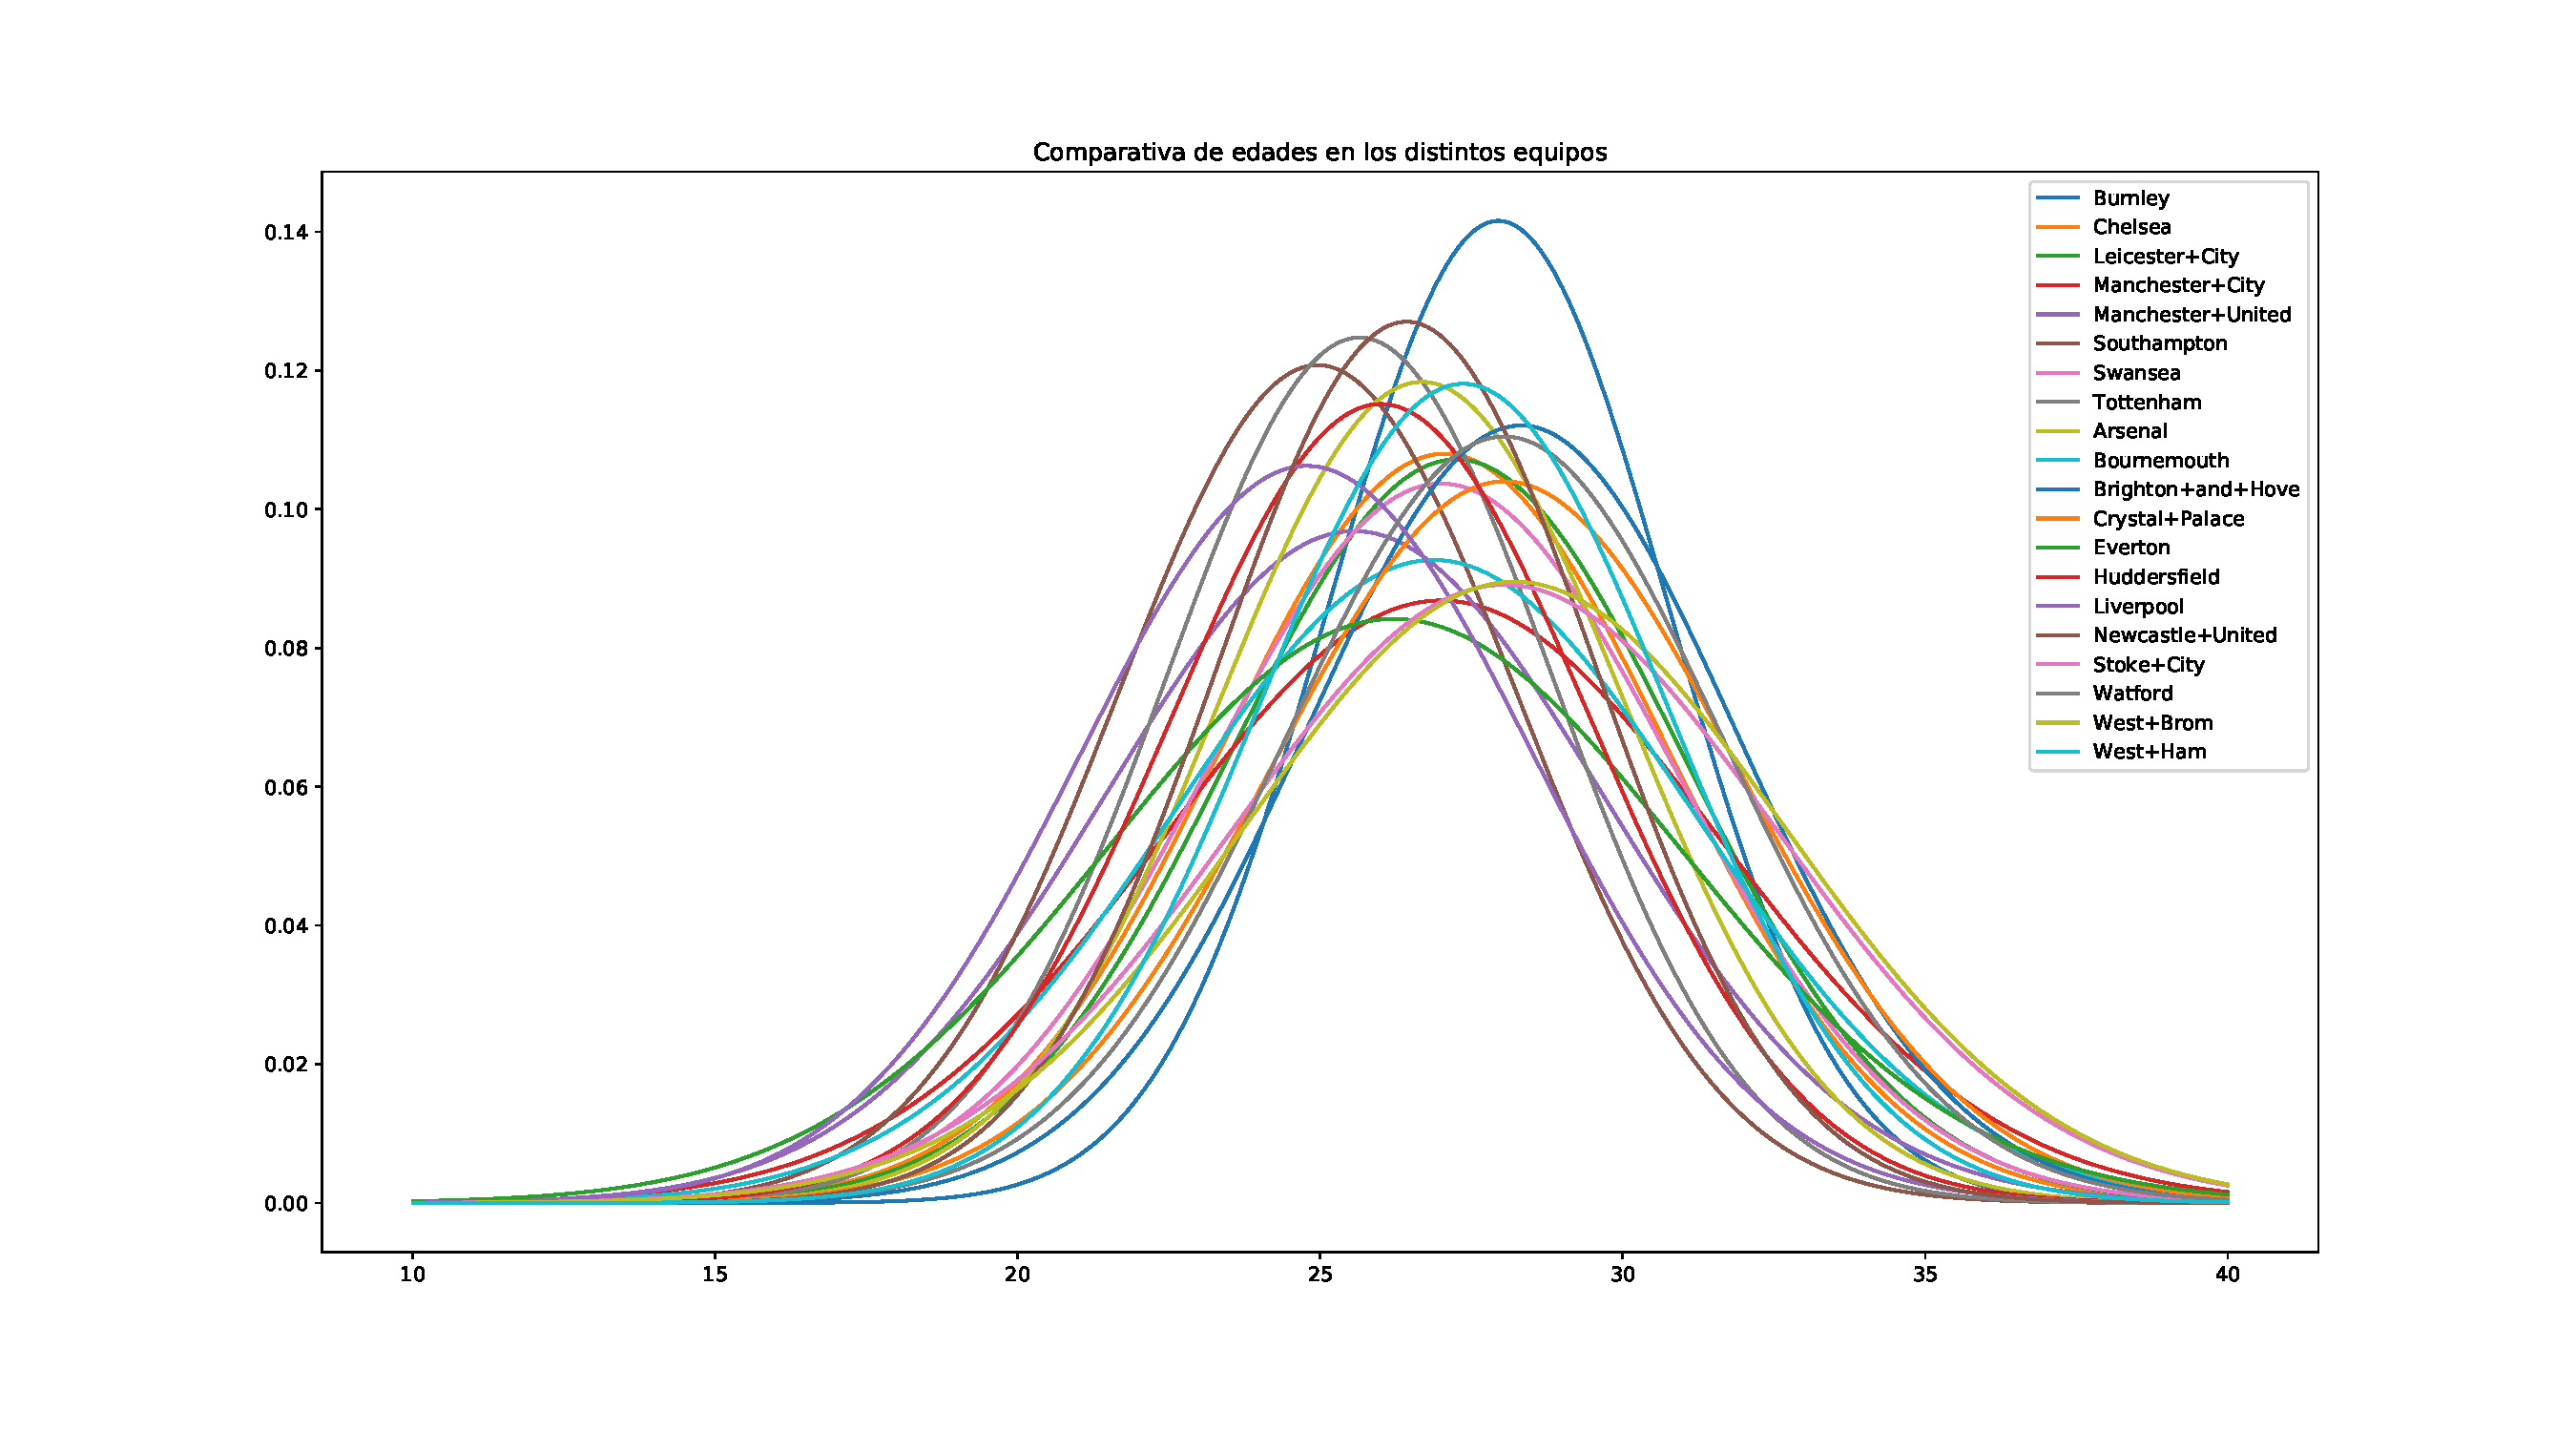
\includegraphics[scale=0.8]{figures/players.pdf}
	\caption{}
\end{figure}

\end{document}
